

\section{Inference with known exposure status}

\paragraph{}Before we look at the reversible-jump mcmc algorithm (RJMCMC),\cite{Green1995-kh} we will show simulation recovery in a simplified framework where we assume the exposure status of every individual (represented by vector $\mathbf{E}$) and exposure time (represented by vector $\mathbf{E^\tau}$) is known. Though knowing this information is rarely feasible in practice, working through this example will help explain how the inference on the fitted parameters $\theta$ and infection state $\mathbf{I}$ work without needing to describe the more complex inference using RJMCMC. 

\subsection{Mathematical representation of framework}

\paragraph{}Let the binary vector $\mathbf{E} = \{ E_1, E_2, \dots, E_M\}$, represent the exposure status of each individual $j$ where $E_j = 0$ is not exposed and $E_j = 1$ is exposed and let $n_\mathbf{E} = \sum_{j = 1}^ME_j$ be the number of exposed individuals. Then, let the vectors $\mathbf{E}^\tau = \{E_1^\tau, E_2^\tau, \dots, E^\tau_{n_\mathbf{E}}\}$ and $\mathbf{I} = \{I_1, I_2^, \dots, I_{n_\mathbf{E}}\}$ be the timing of the exposure and the infection state respectively for each individual which is exposed. The infection state is a binary vector where $I_j = 0$ is not infected, and $I_j = 1$ is infected. Let $Z_{j, t} \in \mathbf{Z}$ represent the dataset of titre values for individual $j$ and at time $t$. 

\paragraph{}We define several functions to help us calculate the likelihood of our model. First, we assume that the model predicted antibody titre at time $t$ in the study ($X_{j.t}$) can be derived given the infection status $I_j$ and timing of exposure $E_j^\tau$. If a person is not infected, their starting titre value ($Z^0_i$) remains unchanged from the start of the study. If the person is infected, their titre remains unchanged until the point of infection, at which point they follow the dynamics highlighted in \textbf{Equation~\ref{eq_ab2}}. The deterministic function for calculating $X_{j,t}$ value is given by

\begin{equation}
\label{eq:ll_abkin}
X_{j,t}  = F_{ab}( I_j,  E_j^\tau, \theta_{ab}, Z^0_j) = 
	\begin{cases}
	Z^0_j + f_{ab}(t - E_j^\tau, \theta_{ab}, Z^0_j),  & \text{If $I_j = 1$, $E_j = 1$, and $t > E_j^\tau$} \\
	Z^0_j, & \text{Otherwise} \\ 
	\end{cases}
\end{equation}

Where $\theta_{ab} = \{a, b, c, \alpha\}$. Second, we define a likelihood function for the correlate of protection. For an individual $j$, with $E_j = 1$, the correlate of protection given exposure at time $t$ with titre value $X_{j, t}$, is assumed to follow a Bernoulli distribution with the probability is given by Equation~\ref{eq_cop}. The PDF of this likelihood is given by Equation~\ref{eq:ll_cop}.

\begin{equation}
\label{eq:ll_cop}
P_{cop}(I_j \mid Z_{j}^0, \theta_{cop} ) =  f_{cop}(Z_{j}^0,  \theta_{cop})^{I_j}(1- f_{cop}(Z_{j}^0,  \theta_{cop} ))^{1-I_j}
\end{equation}

\paragraph{}$\theta_{cop} = \{\beta_0, \beta_1\}$. Finally, we define an observational model to capture variability between hosts and measurement error. Given $X_{j.t}$ and the serological antibody data at the same time point is given by $Z_{j, t}$, we assume the measurement error follows a normal distribution with a PDF given by Equation~\ref{eq:ll_obs}.

\begin{equation}
\label{eq:ll_obs}
P_{obs}(Z_{j,t} \mid X_{j,t}, \sigma) = \frac{1}{\sigma \sqrt{2\pi}} \, e^{-\left(\frac{(Z_{j,t} - X_{j,t})^2}{2\sigma^2}\right)}
\end{equation}

Let $\theta = \{a, b, c, \alpha, \beta_0, \beta_1, \sigma\}$ be the set of continuous parameters which are to be fitted in the model. 

\subsection{Posterior distribution via Bayes rule}

We have two different likelihoods depending on whether an individual is exposed ($E_i = 1$) or not ($E_i = 0$).

\subsubsection{Likelihood for an non exposed individual $E_j = 0$} 
In this case, the value of the timing of exposure and infection status is not applicable and thus not inferred. The likelihood for individual $j$ with serological samples taken at times $t\in T_j$ is therefore equivalent to:
\begin{equation}
\label{ll:1E0}
L_{E_j = 0}(Z_{j}| \theta) = \prod_{t \in T_j}P_{obs}(Z_{j,t}|Z^0_{j}, \sigma)
\end{equation}
as $X_{j.t} = Z^0_{j}$ for all $t$.


\subsubsection{Likelihood for an exposed individual $E_j = 1$}
In this case, the infectious status is determined by the correlate of the protection likelihood ($P_{cop}$) and the antibody kinetics. The likelihood for this individual with serological samples taken at times $t\in T_j$ and infection time $E^\tau_j$ is therefore equivalent to:

\begin{equation}
\label{ll:1E1}
L_{E_j = 1}(Z_{j}| I_j, \theta) = \prod_{t \in T_j}P_{obs}(Z_{j,t}| X_{j,t}, \sigma)P_{cop}(I_j \mid Z_{j}^0, \theta_{cop})
\end{equation}

where $X_{j,t} = F_{ab}( I_j,  E_j^\tau, \theta_{ab}, Z^0_j)$.


\subsubsection{Total likelihood}

If $\mathbf{E_0}$ and $\mathbf{E_1}$ are vectors representing the set of individuals who are not exposed and exposed, respectively. Then, the total likelihood can be written 

\begin{equation}
L(\mathbf{Z} | \mathbf{I}, \theta) = \prod_{j \in \mathbf{E_0}}L_{E_j = 0}(Z_{j}| \theta) \prod_{j \in \mathbf{E_1}}L_{E_j = 1}(Z_{j}| I_j, \theta) 
\end{equation}


\subsubsection{Prior distributions}

\paragraph{}We choose prior distributions for each parameter \pi($\theta$). \textbf{Table~\ref{tab:priorsA}} summarises the chosen priors with their support. 

\begin{table}[ht]
    \centering
    \begin{tabular}{|l|l|l|}
        \hline
        \textbf{Parameter} & \textbf{Prior ($\pi$)} & \textbf{Support ($\mathcal{S}$)} \\
        \hline
        a & $\mathcal{N}(1.5, 0.5)$ & $[0.5, 4]$ \\
        \hline
        b & $\mathcal{N}(0.3, 0.05)$ & $[0, 1]$ \\
        \hline
        c & $\mathcal{U}(0, 4)$ & $[0, 4]$ \\
        \hline
        $\alpha$ & $\mathcal{U}(0, 1)$ & $[0, 1]$ \\
        \hline
        $\beta_0$ & $\mathcal{U}(-10, 10)$ & $[-10, 10]$ \\
        \hline
        $\beta_1$ & $\mathcal{U}(-10, 10)$ & $[-10, 10]$ \\
        \hline
        $\sigma$ &  $\mathcal{U}(0.01, 1)$ & $[0.01, 1]$ \\
        \hline
    \end{tabular}
    \caption{Table with Headers: Parameter, Prior, and Support}
    \label{tab:priorsA}
\end{table}

\paragraph{}We also choose the prior for the number of infections $n_\mathbf{I}$ given the number of exposed individuals $n_\mathbf{E}$ to be a Beta Binomial distribution: $\pi(\mathbf{I}) = \text{BetaBinomial}(n_\mathbf{I} | n_\mathbf{E}, 1, 1)$. Choosing this prior prevents any implicit priors that might rise from products of Bernoulli trials\cite{Hay2020-pr} as $\text{BetaBinomial}(n_\mathbf{I} | n_\mathbf{E} 1, 1) = 1 / n_\mathbf{E}$ for all $0 \leq n_\mathbf{I} \leq n_\mathbf{E}$. 


\subsubsection{Posterior distributions}

\paragraph{}Bayes' rule stipulates that the product of the prior distribution and likelihood is proportional to the posterior distribution; we can use this rule to approximate the posterior for use in the metropolis algorithm. Specifically 

\begin{equation}
\label{eq:bayes}
P(\theta, \mathbf{I} | \mathbf{Z}) \propto \mathcal{L}(\mathbf{Z} | \mathbf{I}, \theta)\pi(\theta)\pi(\mathbf{I})
\end{equation}


\subsection{Metropolis-Hasting algorithm}

\subsubsection{Overview}
\paragraph{} The Metropolis-Hastings. (MH) algorithm is a widely used method for generating samples from a target probability distribution. It falls under the broader category of Markov Chain Monte Carlo (MCMC) methods and is particularly useful when direct sampling from the desired distribution is challenging or impossible such as the likelihood described above. A Markov chain-based approach that iteratively generates a sequence of samples, which eventually converge to the desired distribution. 

\paragraph{}Say we wish to sample from an intractable probability distribttion $P(x)$. The idea of the MH is to define a Markov chain so that the stationary distribution of the Markov chain is $P(x)$. That is, the resulting Markov chain from MH generates a sequence of values, denoted $\{x_1, x_2, \dots,  x_n\}$, such that as $n \rightarrow \infty$ we can guarantee that $x_i \sim P(x)$. To do this, we uniquely define the Markov chain by it's transition probabilities from $x$ to $x'$, $F(x', x)$, that must satisfy the detailed balance condition:

\begin{equation}
\label{eq:db}
F(x' \mid x)P(x)=  F(x\mid x')P(x')
\end{equation}

\paragraph{}This condition ensures that the i) probability density for the next step of the Markov chain is the same as the current density and that ii) this probability density is equal to the posterior.  To construct a transition probability which satisfies this condition, we split $P$ into a proposal distribution $q(x' | x)$ and an acceptance probability $\alpha(x, x')$:

\begin{equation}
F(x' \mid x) = q(x' | x)\alpha(x, x')
\end{equation}

A common choice for $\alpha(x, x')$, which satisfies the detailed balance condition, is the acceptance ratio given by 

\begin{equation}
\label{eq:alpha}
        \alpha(x, x') = \min\left(1, \frac{P(x')}{P(x)} \cdot \frac{Q(x \mid x')}{Q(x' \mid x)}\right)
 \end{equation}

With this, the user has a choice over the proposal distribution $Q$, which can be tailored to optimise the general algorithm given in \textbf{Algorithm~\ref{alg:metropolis_hastings}}.

\begin{algorithm}[H]
\caption{Generic Metropolis-Hastings Algorithm}
\label{alg:metropolis_hastings}
\begin{algorithmic}[1]
    \State Initialize the chain with an initial state $\theta^{(0)}$
    \For{$i = 1$ to $N$}
        \State Generate a candidate state $\theta'$ from the proposal distribution: $\theta' \sim Q(\cdot | \theta^{(i)})$
        \State Compute the acceptance ratio:
        \[
        \alpha(\theta^{(i)}, \theta') = \min\left(1, \frac{P(\theta')}{P(\theta^{(i)})} \cdot \frac{Q(\theta^{(i)} \mid \theta')}{Q(\theta' \mid \theta^{(i)})}\right)
        \]
        \State Sample $u \sim \mathcal{U}(0, 1)$
        \If{$u \leq \alpha$}
            \State Accept the candidate state: $\theta^{(i+1)} \leftarrow \theta'$
        \Else
            \State Reject the candidate state: $\theta^{(i+1)} \leftarrow \theta^{(i)}$
        \EndIf
    \EndFor
\end{algorithmic}
\end{algorithm}



\subsubsection{MH for serological inference with known exposure }

\paragraph{}In our model, we wish to sample from the posterior density function given by \textbf{Equation~\ref{eq:bayes}}, which infers $\theta$, and infectious statuses ${I_j} \in \mathbf{I}$, for $1 \leq j \leq M$ individuals. For the proposal distribution, we define independent proposal distribution for $\theta$ and $\mathbf{I}$,  such that $Q(\cdot | \theta, \mathcal{I}) = q_\theta(\cdot |\theta)q_I(\cdot |\mathbf{I})$. At Markov chain step $i$, we have a value of the parameter space, $\theta^{(i)}$, and propose a new set of parameters $\theta'$ via the proposal distribution $\theta \sim q_\theta(\cdot | \theta^{(i)}, \psi^{(i)}_{adapt})$. This proposal is a multivariate normal distribution with an adaptive covariance matrix, which is defined by the set of parameters $\psi^{(i)}_{adapt}$, which are updated at each time step.\cite{Roberts2012-ju, Andrieu2008-yx} (See Appendix). For $\mathbf{I}$, we propose a new infection state $\mathbf{I}'$ by selecting an exposed individual $j$, which has infection status $I_j^{(i)}$ at step $i$ of the current Markov chain, we sample a proposal value for their infection status $I_j'$ by the proposal distribution for $I_j' \sim q_I(\cdot | I^{(i)}_j)= \text{Bernoulli(0.5)}$. Therefore the proposal for $q_I(\mathbf{I}'|\mathbf{I}) = 1/n_\mathbf{E}0.5$ for all $j$. Both of these proposals $q_\theta\left(\theta' | \theta^{(i)}, \psi^{(i)}_{adapt}\right)$, $q_I(\mathbf{I}'|\mathbf{I})$ are both symmetric and thus cancel out the acceptance ratio (\textbf{Equation~\ref{eq:alpha}}). Further, the prior distribution $\pi(\mathbf{I}) = 1 / n_\mathbf{E}$ for all $0 \leq n_\mathbf{I} \leq n_\mathbf{E}$, and thus also cancels out in the acceptance ratio, therefore we need only calculate: $P(\theta, \mathbf{I} | \mathbf{Z}) \propto \mathcal{L}(\mathbf{Z} | \mathbf{I}, \theta)\pi(\theta)$

\paragraph{}Consequently, we construct a new algorithm for inference of the known exposure model (\textbf{Algorithm~\ref{alg:metropolis_hastings_inf}}).

\begin{algorithm}[H]
\caption{Metropolis-Hastings Algorithm for antibody kinetics and infection inference}
\label{alg:metropolis_hastings_inf}
\begin{algorithmic}[1]
    \State Initialize the chain with an initial state $\theta^{(0)}$ from the priors $\pi(\cdot)$ and $I^{(0)}_{j} \sim \text{Bernoulli(0.5)}$ for all $1 \leq j \leq M$ individuals to intialise $\mathbf{I}^{(0)}$, and initialise $\psi^{(0)}_{adapt}$.
    \For{$i = 1$ to $N$}
        \State Generate a candidate state $\theta' \sim q_\theta\left(\theta^{(i)}, \psi^{(0)}_{adapt}\right)$
        \State Generate a candidate individual $j \in \mathbf{E_1} $, then a candidate state $I'_j \sim \text{Bernoulli(0.5)}$ to propose $\mathbf{I}'$
        \State Compute the acceptance ratio:
        \[
        \alpha((\theta^{(i)}, \mathbf{I}^{(i)}),( \theta',  \mathbf{I}')) = \min\left(1, \frac{P(\theta', \mathbf{I}'|\mathbf{Z})}{P(\theta^{(i)}, \mathbf{I}^{(i)}|\mathbf{Z})} \right)
        \]
        \State Sample $u \sim \mathcal{U}(0, 1)$
        \If{$u \leq \alpha$}
            \State Accept the candidate state: $\theta^{(i+1)} \leftarrow \theta'$ and $\mathbf{I}^{(i + 1)}  \leftarrow \mathbf{I}'$
        \Else
            \State Reject the candidate state: $\theta^{(i+1)} \leftarrow \theta^{(i)}$ and $\mathbf{I}^{(i + 1)}  \leftarrow \mathbf{I}^{(i)} $
        \EndIf 
        \State Update $ \psi^{(i + 1)}_{adapt} \leftarrow \psi^{(i)}_{adapt}$
    \EndFor
\end{algorithmic} 
\end{algorithm}


\subsection{Implementation }
\paragraph{}  \textbf{Algorithm~\ref{alg:metropolis_hastings_inf}} is coded manually in R and cpp through Rcpp. We run the algorithm for four chains, each with 200,000 steps, with 100,000 burn-ins steps. The initial values for $\theta$ and $\mathbf{I}$ are sampled from their prior distributions. We initialise the adaptive covariance by running with an identity matrix with each parameter scale according to 1,000 steps, then sample from the adaptive scheme. (see \textbf{Appendix}). We thin the posterior samples by taking one in every 100, leaving 1,000 posterior samples at the end of the sampling.

\subsection{Simulation recovery }
\paragraph{} After running \textbf{Algorithm~\ref{alg:metropolis_hastings_inf}}, we plot the posterior samples, $\hat{\theta}$ and $\hat{\mathbf{I}}$ and compare with the simulated parameters.

\subsubsection{Infection recovery}

\paragraph{}We assess the ability of the algorithm to recover the infection status of each individual in the study. If the set posterior samples of the infection status for individual $j$ is given by $\hat{I_j} $, then we plot the expectation $\mathbb{E}[\hat{I_j}]$ so we can assess the ability of the algorithm to recover the individual-level simulated infection status (\textbf{Figure~\ref{fit1:inf}}). Given no COP model A, we find when the pre-infection titre is less than 3.3 that all six models considered can recover the infection status of almost all individuals. When the pre-infection titre is greater than 3.3, the attenuation of boosting for infected individuals causes no meaningful change in the antibody kinetics ($f^2_{ab}(Z, \alpha) = 0$ when $Z > 3.3$). Thus, these individuals' infections are difficult to infer serologically as their titre dynamics are equivalent and independent of their infection status. In our COP model B, we find that including the correlate of protection influences the infection status. As the inferred correlate (\textbf{Figure~\ref{fit1:cop}}) has a low probability of infection at higher titres, this causes the $\mathbb{E}[\hat{I_j}]$ to be more likely to be 0 at higher titre values. Thus, the infection statuses for nearly all individuals are recoverable for COP model B.

\begin{figure}[H]
    \centering
    \begin{subfigure}{0.31\textwidth}
        \centering
        \includegraphics[width=\textwidth]{\myimagepath/outputs/fits/cesNoCOP/knownExp/figs/obs_0.1/infection_recov.png}
        \caption{No COP, 10\% observation error \label{fit1:infA}}
    \end{subfigure}
    \begin{subfigure}{0.31\textwidth}
        \centering
        \includegraphics[width=\textwidth]{\myimagepath/outputs/fits/cesNoCOP/knownExp/figs/obs_0.3/infection_recov.png}
        \caption{No COP, 30\% observation error \label{fit1:infB}}
    \end{subfigure}
    \begin{subfigure}{0.31\textwidth}
        \centering
        \includegraphics[width=\textwidth]{\myimagepath/outputs/fits/cesNoCOP/knownExp/figs/obs_0.5/infection_recov.png}
        \caption{No COP, 50\% observation error \label{fit1:infC}}
    \end{subfigure}
    
  \begin{subfigure}{0.31\textwidth}
        \centering
        \includegraphics[width=\textwidth]{\myimagepath/outputs/fits/cesCOP/knownExp/figs/obs_0.1/infection_recov.png}
        \caption{ COP, 10\% observation error \label{fit1:infD}}
    \end{subfigure}
    \begin{subfigure}{0.31\textwidth}
        \centering
        \includegraphics[width=\textwidth]{\myimagepath/outputs/fits/cesCOP/knownExp/figs/obs_0.3/infection_recov.png}
        \caption{ COP, 30\% observation error \label{fit1:infE}}
    \end{subfigure}
    \begin{subfigure}{0.31\textwidth}
        \centering
        \includegraphics[width=\textwidth]{\myimagepath/outputs/fits/cesCOP/knownExp/figs/obs_0.5/infection_recov.png}
        \caption{ COP, 50\% observation error \label{fit1:infF}}
    \end{subfigure}
    
    \caption{Simulation recovery of the individual infection status, $\mathbb{E}[\hat{I_j}]$, for two COP models (top: No COP, bottom: logistic COP) and three different levels antibody kinetics variability (10\%, 30\%, 50\%) \label{fit1:inf}}
\end{figure}


\subsubsection{Correlate of protection}

\paragraph{}We next assess the ability of \textbf{Algorithm~\ref{alg:metropolis_hastings_inf}} to recover the correlate of protection function $f_{cop}(x, \hat{\theta}_{cop})$, where $x$ is the titre value at infection and where $\hat{\theta}_{cop} = \{\hat{\beta_0}, \hat{\beta_1}\}$ are the posterior samples for $\beta_0$ and $\beta_1$. We consider two COP models: COP model A, no correlate of protection, and COP model B, a logistic curve for COP. For Model A, we find that the COP curve is mostly recovered, with the simulated line within a 95\% confidence interval of the posterior sample (\textbf{Figure~\ref{fit1:cop}}). For Model B, we also find the logistic shape of the COP is recovered in the posterior samples. The variability in the antibody kinetics seemed to have a negligible effect on the recoverability of the COP curve. To understand the difference between the simulated functional form in \textbf{Figure~\ref{fit1:cop}} in red, and the posterior samples, we have plotted the inferred COP from the simulated infection states in \textbf{Figure~\ref{fig:sim_C}}. Here, it is clear that although we have a pre-defined function for the correlate of protection, when we simulate the data the COP curve is not perfectly recovered. Thus, the posterior distribution of our inference method can, at best, recover the inferred COP curve.

\begin{figure}[H]

    \centering
    \begin{subfigure}{0.31\textwidth}
        \centering
        \includegraphics[width=\textwidth]{\myimagepath/outputs/fits/cesNoCOP/knownExp/figs/obs_0.1/cop_recov.png}
        \caption{No COP, 10\% observation error \label{fit1:copA}}
    \end{subfigure}
    \begin{subfigure}{0.31\textwidth}
        \centering
        \includegraphics[width=\textwidth]{\myimagepath/outputs/fits/cesNoCOP/knownExp/figs/obs_0.3/cop_recov.png}
        \caption{No COP, 30\% observation error \label{fit1:copB}}
    \end{subfigure}
    \begin{subfigure}{0.31\textwidth}
        \centering
        \includegraphics[width=\textwidth]{\myimagepath/outputs/fits/cesNoCOP/knownExp/figs/obs_0.5/cop_recov.png}
        \caption{No COP, 50\% observation error \label{fit1:copC}}
    \end{subfigure}
    
  \begin{subfigure}{0.31\textwidth}
        \centering
        \includegraphics[width=\textwidth]{\myimagepath/outputs/fits/cesCOP/knownExp/figs/obs_0.1/cop_recov.png}
        \caption{ COP, 10\% observation error \label{fit1:copD}}
    \end{subfigure}
    \begin{subfigure}{0.31\textwidth}
        \centering
        \includegraphics[width=\textwidth]{\myimagepath/outputs/fits/cesCOP/knownExp/figs/obs_0.3/cop_recov.png}
        \caption{ COP, 30\% observation error \label{fit1:copE}}
    \end{subfigure}
    \begin{subfigure}{0.31\textwidth}
        \centering
        \includegraphics[width=\textwidth]{\myimagepath/outputs/fits/cesCOP/knownExp/figs/obs_0.5/cop_recov.png}
        \caption{ COP, 50\% observation error \label{fit1:copF}}
    \end{subfigure}
    
    \caption{Simulation recovery of the COP function, with posterior samples plot  $f_{cop}(x, \hat{\theta}_{cop})$. We have two different COP models (top: No COP, bottom: logistic COP) and three different levels of antibody kinetics variability (10\%, 30\%, 50\%). \label{fit1:cop}}
    \end{figure}


\subsubsection{Antibody kinetics}

\paragraph{} \textbf{Algorithm~\ref{alg:metropolis_hastings_inf}} also succesfully recovers the simualted antibody kinetics. Let us plot $f^1_{ab}(s, \hat{a}, \hat{b}, \hat{c})$, the posterior predictive distribution for the antibody kinetic boosting, given posterior distributions  $\hat{a}, \hat{b}$, and $\hat{c}$. At all three levels of kinetic uncertainty, the antibody kinetics are recovered, though increasing uncertainty weakens the accuracy of the recovered curves compared to the simulated. (\textbf{Figure~\ref{fit1:ab}}).

\begin{figure}[H]
    \centering
    \begin{subfigure}{0.31\textwidth}
        \centering
        \includegraphics[width=\textwidth]{\myimagepath/outputs/fits/cesNoCOP/knownExp/figs/obs_0.1/ab_kinetics_recov.png}
        \caption{No COP, 10\% observation error}
    \end{subfigure}
    \begin{subfigure}{0.31\textwidth}
        \centering
        \includegraphics[width=\textwidth]{\myimagepath/outputs/fits/cesNoCOP/knownExp/figs/obs_0.3/ab_kinetics_recov.png}
        \caption{No COP, 30\% observation error}
    \end{subfigure}
    \begin{subfigure}{0.31\textwidth}
        \centering
        \includegraphics[width=\textwidth]{\myimagepath/outputs/fits/cesNoCOP/knownExp/figs/obs_0.5/ab_kinetics_recov.png}
        \caption{No COP, 50\% observation error}
    \end{subfigure}
    
  \begin{subfigure}{0.31\textwidth}
        \centering
        \includegraphics[width=\textwidth]{\myimagepath/outputs/fits/cesCOP/knownExp/figs/obs_0.1/ab_kinetics_recov.png}
        \caption{ COP, 10\% observation error}
    \end{subfigure}
    \begin{subfigure}{0.31\textwidth}
        \centering
        \includegraphics[width=\textwidth]{\myimagepath/outputs/fits/cesCOP/knownExp/figs/obs_0.3/ab_kinetics_recov.png}
        \caption{ COP, 30\% observation error}
    \end{subfigure}
    \begin{subfigure}{0.31\textwidth}
        \centering
        \includegraphics[width=\textwidth]{\myimagepath/outputs/fits/cesCOP/knownExp/figs/obs_0.5/ab_kinetics_recov.png}
        \caption{ COP, 50\% observation error}
    \end{subfigure}
    
    \caption{Simulation recovery of the antibody kinetics function with posterior samples plot $f^1_{ab}(s, \hat{a}, \hat{b}, \hat{c})$. We have two different COP models (top: No COP, bottom: logistic COP) and three different levels of antibody kinetics variability (10\%, 30\%, 50\%). \label{fit1:ab}
}

\end{figure}



